\documentclass[ngerman]{beamer}
\usepackage{babel}
\usepackage[utf8]{inputenc}
\usepackage[T1]{fontenc}
\usepackage{lmodern}
\usepackage{pstricks}
\usepackage{tikz}
\usetikzlibrary{arrows,automata}

\usetheme{TUC2}
\setbeamercovered{transparent}

\mode<presentation>
\title{Hybride Systeme}
\subtitle{Dependability and Trust}
\author{Daniel Arnsberger und Niklas Fiekas}
\institute{Institut für Informatik}
\date{04. Juli 2014}

\begin{document}

\begin{frame}
    \titlepage
\end{frame}

\begin{frame}
    \frametitle{Inhalt}
    \tableofcontents
\end{frame}

\begin{section}{Sicherheit und Stabilität}

\begin{frame}
    \frametitle{Ein hybrides Szenario}
    \begin{figure}
        \centering
        \def\svgwidth{0.9\columnwidth}
        \input{szenario.pdf_tex}
    \end{figure}
\end{frame}

\begin{frame}
    \frametitle{Sicherheit}
    \begin{figure}
        \centering
        \def\svgwidth{0.9\columnwidth}
        \input{safety.pdf_tex}
    \end{figure}
\end{frame}

\begin{frame}
    \frametitle{Stabilität}
    \begin{figure}
        \centering
        \def\svgwidth{0.9\columnwidth}
        \input{stability.pdf_tex}
    \end{figure}
\end{frame}

\end{section}
\begin{section}{Diskreter Teil der Modellierung}

\begin{frame}
    \frametitle{Endliche Automaten}

    $$\mathcal{F} = \{ \mathit{Loc}, \mathit{Act}_{\mathcal{F}}, \mathit{Edges}, \mathit{loc}_0 \} $$

    \begin{itemize}
        \item $\mathit{Loc} = \{ \blacksquare, \blacktriangle, \circlearrowleft \} $
        \item $\mathit{Act}_{\mathcal{F}} = \{ \text{drive}, \text{turn}, \text{stop} \} $
        \item $\mathit{Edges} \subseteq \mathit{Loc} \times \mathit{Act}_{\mathcal{F}} \times \mathit{Loc} $
        \item $\mathit{loc}_0 \in \mathit{Loc} $
    \end{itemize}
\end{frame}

\begin{frame}
    \frametitle{Endliche Automaten}
    \begin{figure}
        \centering
        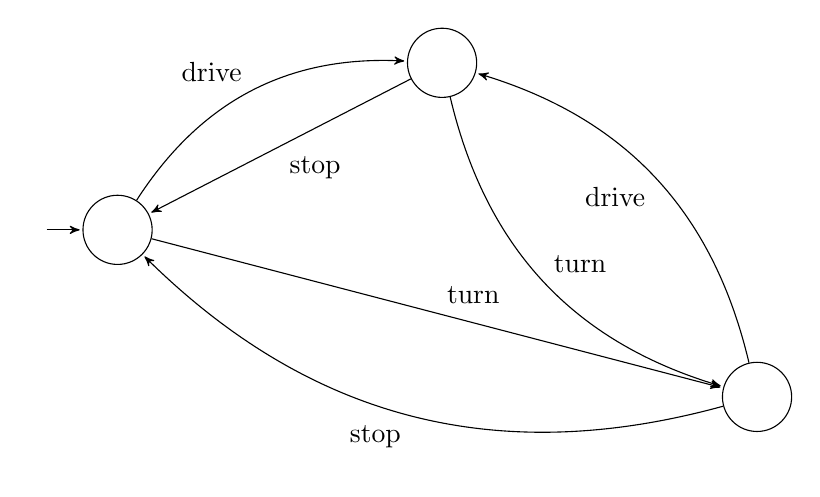
\begin{tikzpicture}[->,>=stealth',shorten >=1pt,auto,node distance=3cm]
            \node[state,initial,initial text={}] (off) {$\blacksquare$};
            \node[state,xshift=2cm] (driving) [above right of=off] {$\blacktriangle$};
            \node[state,xshift=6cm] (turning) [below right of=off] {$\circlearrowleft$};

            \path (off)     edge [bend left]  node {drive} (driving)
                  (off)     edge              node {turn}  (turning)
                  (turning) edge [bend left]  node {stop}  (off)
                  (turning) edge [bend right] node {drive} (driving)
                  (driving) edge              node {stop}  (off)
                  (driving) edge [bend right] node {turn}  (turning);
        \end{tikzpicture}
    \end{figure}

\end{frame}

\end{section}
\begin{section}{Kontinuierlicher Teil der Modellierung}

\begin{frame}
    \frametitle{Hybride Automaten}

    \begin{align*}
        \mathcal{H} = \{ & \mathit{Loc}, \mathit{Act}_{\mathcal{H}}, \mathit{Edges}, \mathit{loc}_0, \\
                         & \mathit{Cont}, \mathit{Cont}_0, \mathit{inv}, \mathit{flow}, \mathit{guard}, \mathit{reset} \}
    \end{align*}
\end{frame}

\end{section}
\begin{section}{Ausblick}

\begin{frame}
    \frametitle{Ausblick}
\end{frame}

\end{section}
\end{document}
